% =========================================================
% QUESTION 1
% =========================================================
\section{نصب}
در این بخش بدون چالش خاصی داکر\footnote{Docker} بر دستگاه نصب شده و برنامهٔ \lr{hello-world} اجرا شد.
\begin{LTR}
    \begin{minted}{bash}
docker --version
docker info
docker run --rm hello-world
    \end{minted}
\end{LTR}

\begin{figure}[htbp]
    \centering
    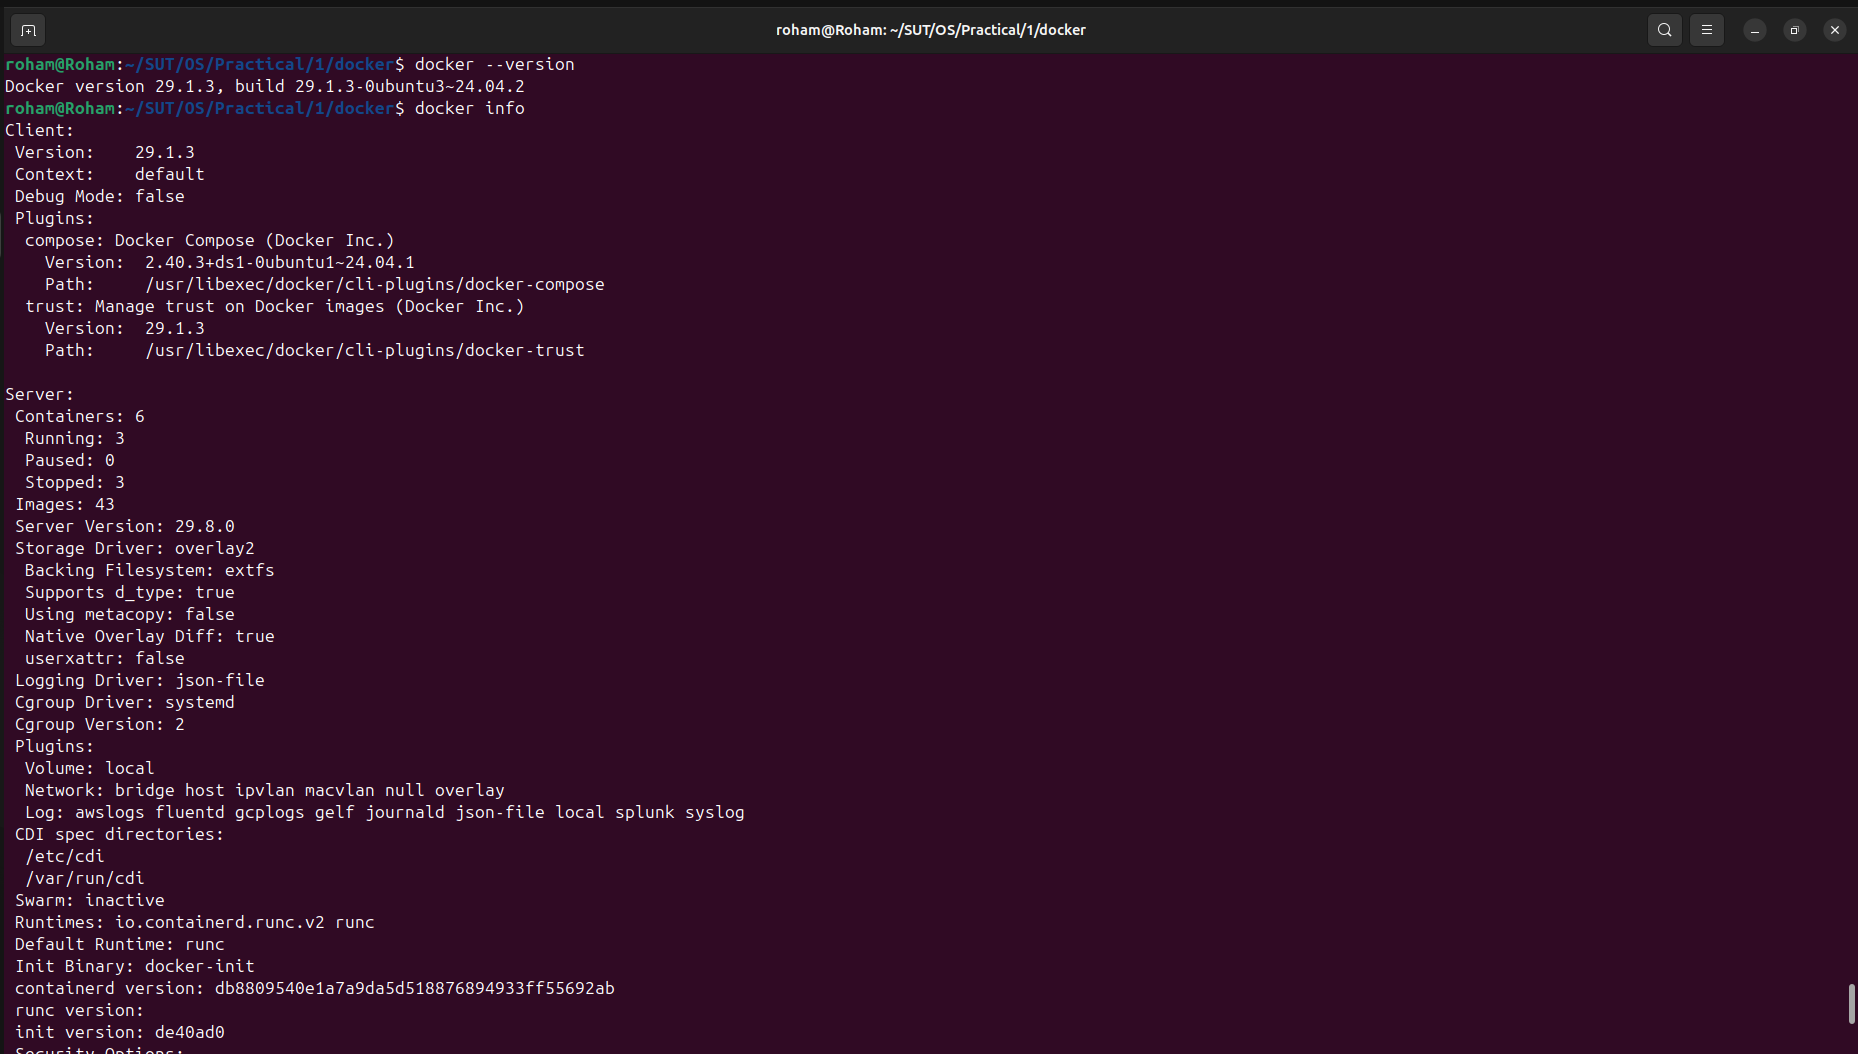
\includegraphics[width=0.8\textwidth]{Images/PHW1.2-Docker Info.png}
    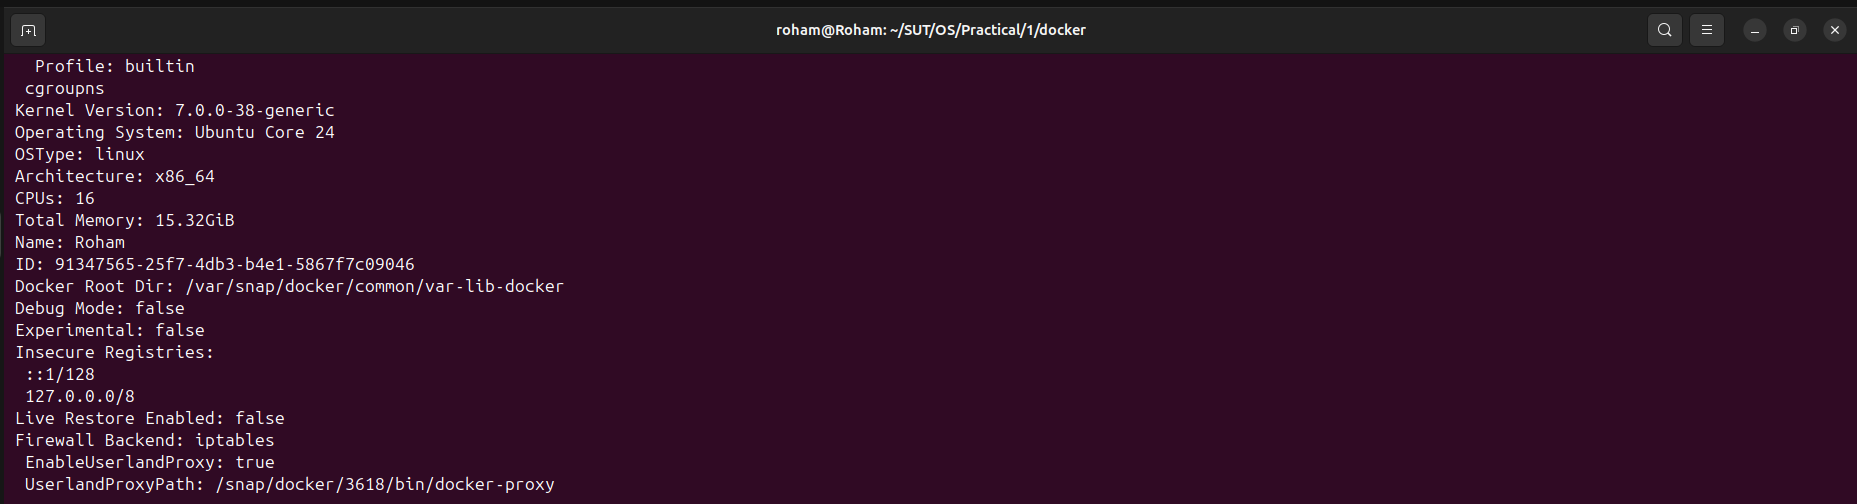
\includegraphics[width=0.8\textwidth]{Images/PHW1.2-Docker Info2.png}
    \caption{بررسی نسخه}
\end{figure}
\begin{figure}[htbp]
    \centering
    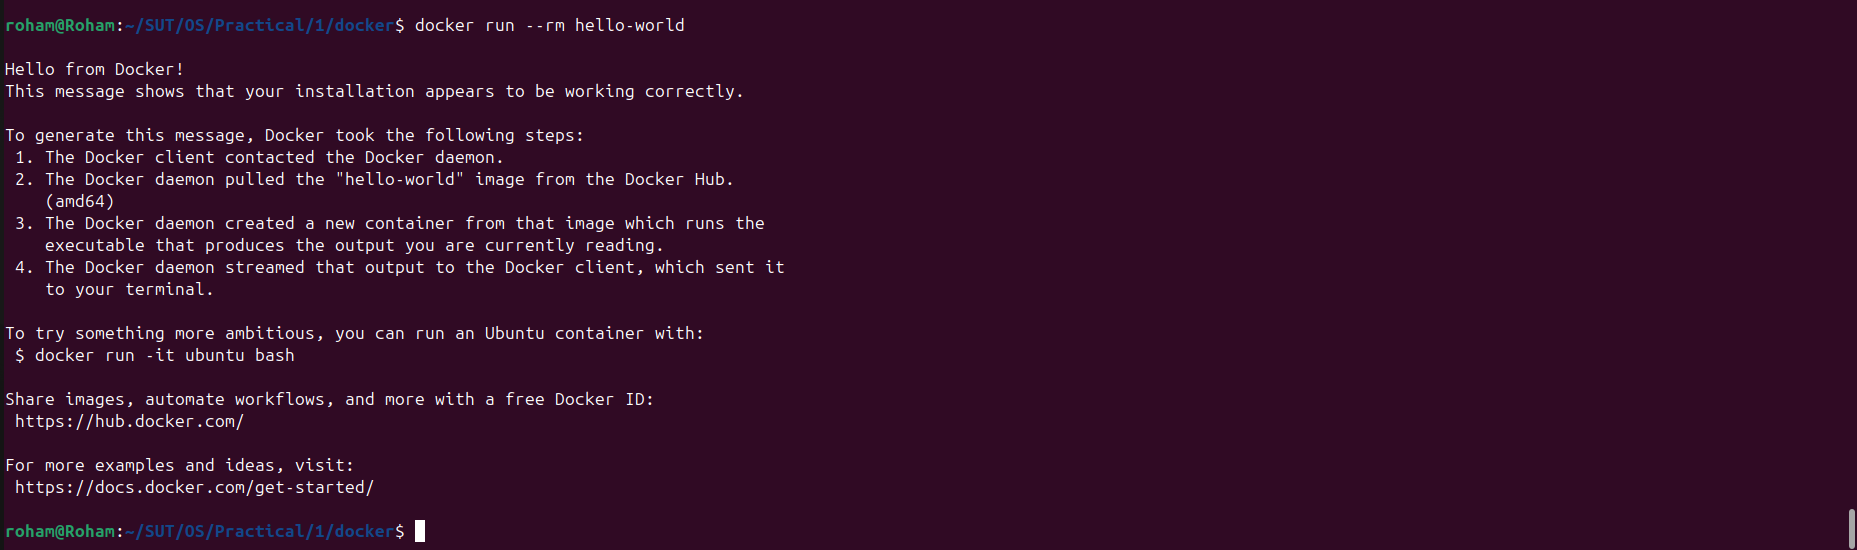
\includegraphics[width=0.8\textwidth]{Images/PHW1.2-Docker Hello world.png}
    \caption{اجرای برنامه \lr{hello-world}}
\end{figure}

\section{تصویر و کانتینر}
در این بخش یک تصویر\footnote{Image} اوبونتو\footnote{Ubuntu} اجرا شده و چند دستور داخل آن بررسی می‌گردد.
\par

\begin{LTR}
    \begin{minted}{bash}
docker pull ubuntu:24.04
docker images
docker run -it --name os ubuntu:24.04 bash
uname -r
caat /etc/os-release
touch /tmp/os.txt
exit
    \end{minted}
\end{LTR}


\begin{figure}[htbp]
    \centering
    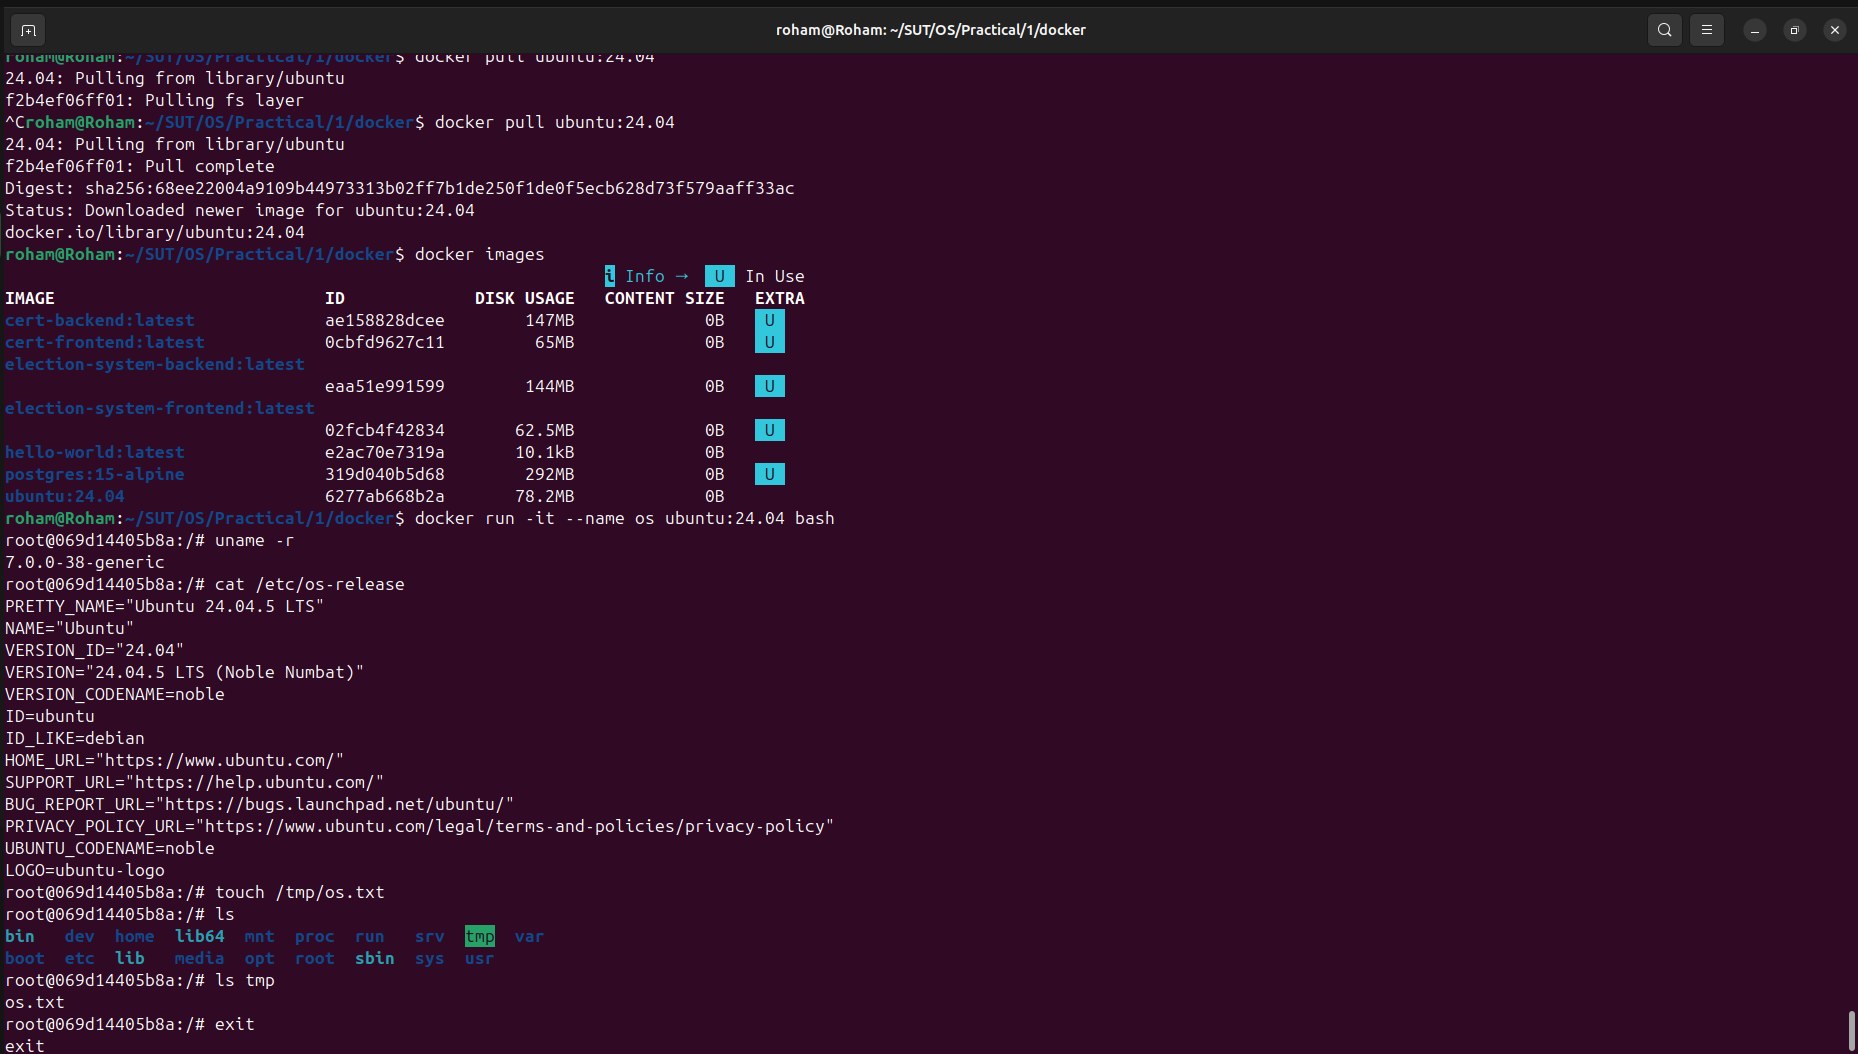
\includegraphics[width=0.8\textwidth]{Images/PHW1.2-2.png}
    \caption{اجرای تصویر اوبونتو}
\end{figure}
\par
در این بخش ابتدا تصویر \lr{ubuntu:24.04} واکشی\footnote{Pull} شده و سپس تصاویر فعلی داکر بررسی می‌شوند؛ قابل
توجه است تعدادی تصویر از پروژه‌های شخصی نیز در کنار تصویر اوبونتو قابل ملاحظه می‌باشد. در ادامه تصویر اوبونتو تحت نام "os"
در داکر اجرا شده‌است و در ادامه برخی دستورات لینوکس در اوبونتوی داخلی اجرا گردیده است.
\par
در این چند دستور برای تغییر فایل‌ها و بررسی فایل‌های داخل سیستم عامل درونی اجرا شده است و برای راستی‌أزمایی دستورات \lr{\mintinline{bash}{ls}}
و خروجی آن‌ها قابل مشاهده می‌باشند.

\section{مدیریت کانتینر}
در این بخش یک تصویر دیگر از اوبونتو اجرا شده و به یکی از این تصاویر دستور \lr{\mintinline{bash}{sleep}} داده شده است
و در این حین وضعیت کانتینر\footnote{Container}ها بررسی می‌گردند و در انتها نیز کانتینرها حذف می‌شوند.
\begin{LTR}
    \begin{minted}{bash}
docker run d --name os-bg ubuntu:24.04 sleep 600
docker ps
docker stop os-bg
docker start os-bg
docker stop os-bg
docker rm os-bg
docker rm os
    \end{minted}
\end{LTR}
\begin{figure}[htbp]
    \centering
    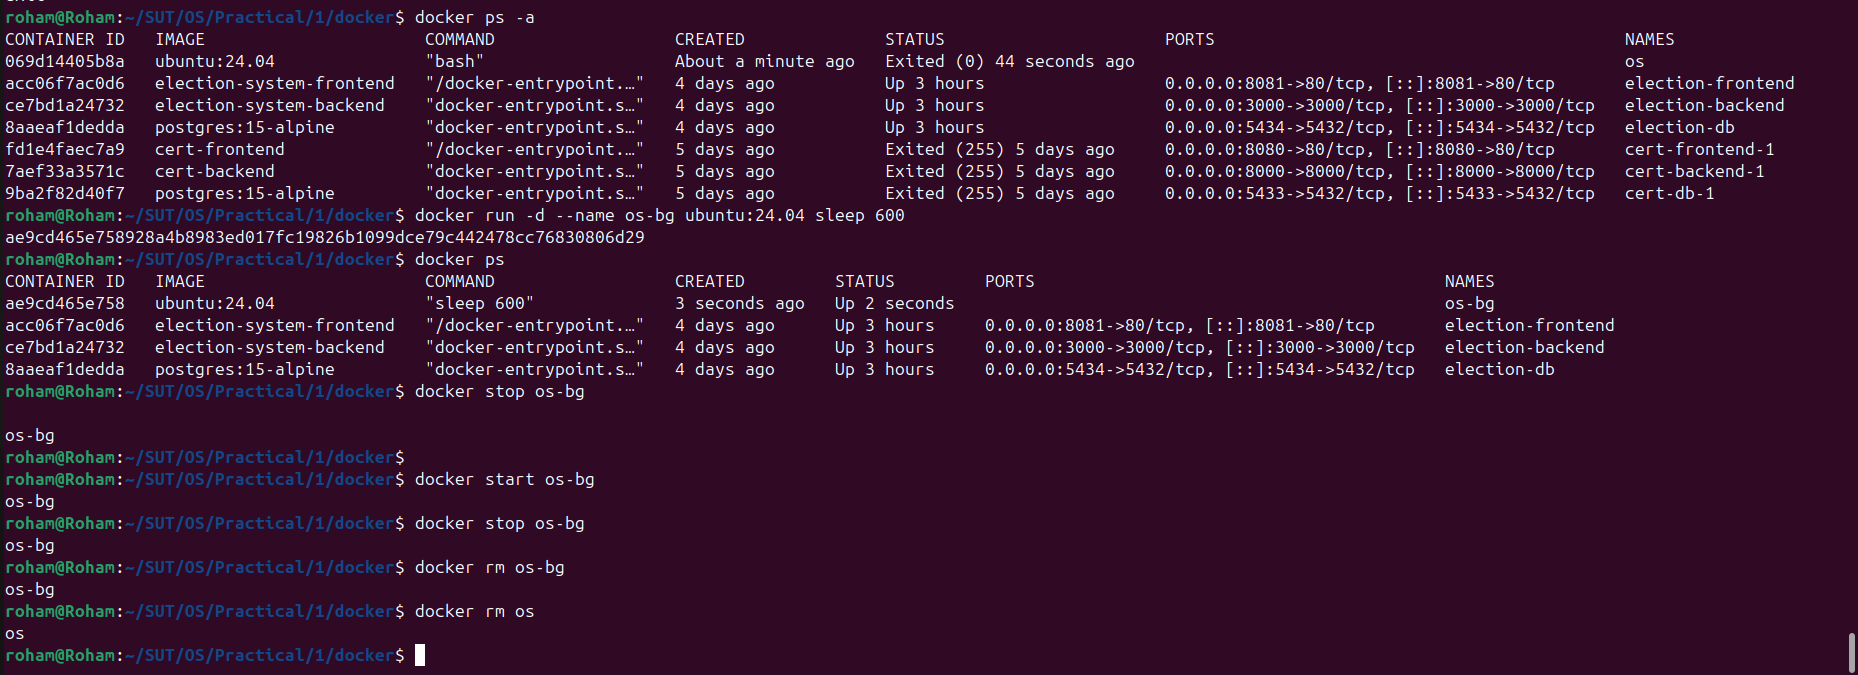
\includegraphics[width=0.8\textwidth]{Images/PHW1.2-3.png}
    \caption{بررسی وضعیت کانتینر‌ها و حذف آنان}
\end{figure}
\subsection{سوال}
تصاویر یک برنامه فقط خواندنی \footnote{\lr{Read-Only}} می‌باشد که شامل برخی‌ کد‌ها و کتابخانه‌ها و تنظیمات پیکربندی\footnote{Configuration Settings} می‌شود
در حالی که کانتینر یک نمونهٔ تصویر درحال اجرا می‌باشد که علاوه بر موارد تصویر، یک لایهٔ قابل نوشتن\footnote{Writable} دارد و به همین دلیل هنگامی که از کانتینر خارج می‌شویم
همچنان آن لایهٔ نوشته شده در حافظه ذخیره می‌شود و پس از راه‌اندازی مجدد داده‌ها بازیابی می‌شوند؛ مگر آن که
کانتینر کاملا حذف گردد.

\pagebreak
\section{مقایسه \lr{Bare Metal}، ماشین مجازی و داکر}
\subsubsection{اطلاعات سیستم \lr{Bare Metal}}
\begin{table}[ht]
    \centering
    \caption{مشخصات سخت‌افزاری و نرم‌افزاری سیستم میزبان (\lr{Bare Metal})}
    \begin{tabular}{|r|l|}
        \hline
        \textbf{مشخصه} & \multicolumn{1}{r|}{\textbf{مقدار}} \\ \hline
        مدل پردازنده & \lr{13th Gen Intel(R) Core(TM) i7-13620H} \\ \hline
        تعداد رشته‌های پردازشی & \lr{16 (NUMA node0: 0--15)} \\ \hline
        حافظه اصلی & \lr{15 GiB} \\ \hline
        توزیع سیستم‌عامل & \lr{Ubuntu 24.04.3 LTS (Noble)} \\ \hline
        نسخه هسته & \lr{7.0.0-38-generic} \\ \hline
    \end{tabular}
\end{table}


\subsubsection{اطلاعات \lr{Docker}}
\begin{table}[ht]
    \centering
    \caption{مشخصات (\lr{Docer})}
    \begin{tabular}{|r|l|}
        \hline
        \textbf{مشخصه} & \multicolumn{1}{r|}{\textbf{مقدار}} \\ \hline
        نسخه & \lr{Docker version 29.1.3, build 29.1.3-0ubuntu3~24.04.2} \\ \hline
        سطخ دسترسی & \lr{Unbound} \\ \hline
    \end{tabular}
\end{table}

\subsubsection{اطلاعات \lr{Virutal Machine}}
\begin{table}[ht]
    \centering
    \caption{مشخصات ماشین مجازی (\lr{VM - Multipass})}
    \begin{tabular}{|r|l|}
        \hline
        \textbf{مشخصه} & \multicolumn{1}{r|}{\textbf{مقدار}} \\ \hline
        توزیع سیستم‌عامل & \lr{Ubuntu 24.04.5 LTS} \\ \hline
        تعداد پردازنده‌های مجازی & \lr{4} \\ \hline
        حافظه رم تخصیص‌یافته & \lr{3.8 GiB ($\approx$ 4 GB)} \\ \hline
        فضای دیسک & \lr{9.6 GiB ($\approx$ 10 GB)} \\ \hline
    \end{tabular}
\end{table}

\subsubsection{اطلاعات \lr{Sysbench}}
در تمامی محیط‌ها از \lr{\mintinline{bash}{sysbench 1.0.20}} استفاده شده است.

\subsection{\lr{CPU Intensive}}
\subsubsection{توضیح محک}
این محک با استفاده از ۴ ریسمان\footnote{ُThread} تلاش می‌کند، اعداد اول بین ۳ تا ۲۰۰۰۰۰۰ را به روش کلاسیک بیابد، و به ندرت به I/O یا حافظه دسترسی خواهد داشت.

\subsubsection{پیش‌بینی}
با توجه به اینکه دسترسی به حافظه و I/O ناچیز است، پیش‌بینی می‌شود که
هر سه محیط اجرا عملکرد نسبتا مشابهی در ۹۹ صدک برتر داشته باشند، به طور میانگین ممکن است که
در ماشین مجازی بدلیل سرباز مجازی سازی ناشی مدیریت وقفه‌های مجازی تاخیر افزایش داشته باشد.

\subsubsection{شبیه‌سازی}
\begin{figure}[ht]
    \centering
    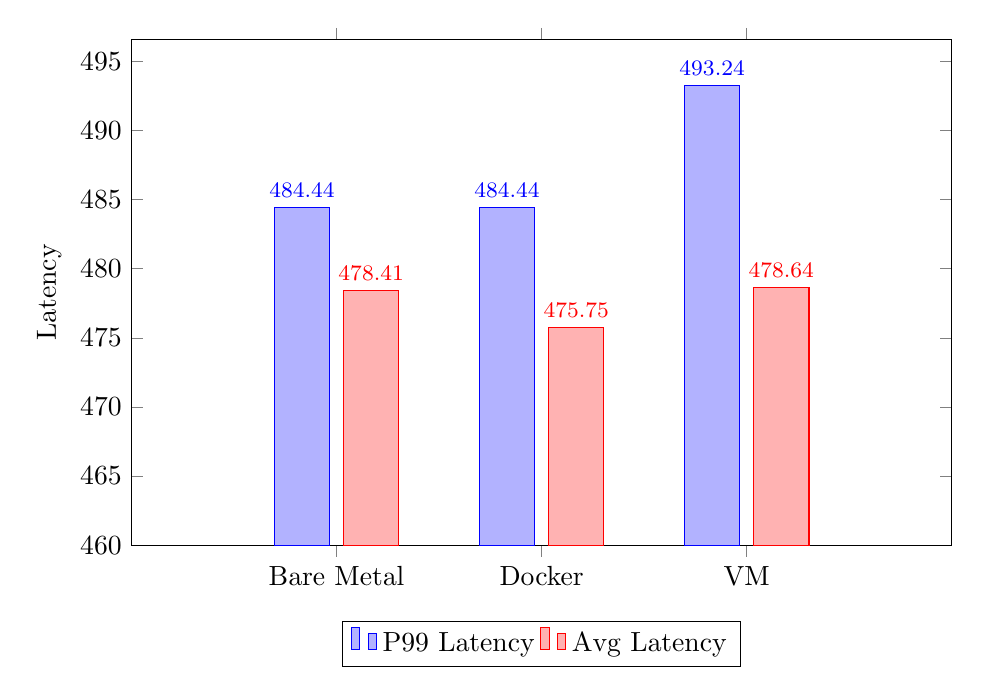
\begin{tikzpicture}
        \begin{axis}[
            ybar=5pt,
            bar width=20pt,
            width=12cm,
            height=8cm,
            enlarge x limits=0.5,
            ymin=460, 
            ylabel={Latency},
            symbolic x coords={Bare Metal, Docker, VM},
            xtick=data,
            nodes near coords,
            nodes near coords align={vertical},
            nodes near coords style={font=\footnotesize},
            legend style={at={(0.5,-0.15)}, anchor=north, legend columns=-1},
        ]
        
        \addplot coordinates {(Bare Metal, 484.44) (Docker, 484.44) (VM, 493.24)};
        \addplot coordinates {(Bare Metal, 478.41) (Docker, 475.75) (VM, 478.64)};
        
        \legend{\lr{P99} Latency, Avg Latency}
        \end{axis}
    \end{tikzpicture}
    \caption{مقایسه با بنچمارک \lr{CPU Intensive}}
\end{figure}

\subsubsection{تحلیل نتایج}
همانطور که مشاهده می‌شود در ۹۹ صدک، داکر و \lr{Bare Metal} عملکرد و مشابهی داشته‌اند و ماشین مجازی
ضعیف‌تر عمل کرده است که مشابه پیش‌بینی می‌باشد. همچنین در میانگین هم همانطور که پیش‌بینی شده است، ماشین مجازی ضعیف‌ترین عملکرد را داشته است.
البته داکر عملکرد خیلی بهتری نسبت به دو محیط دیگر داشته است که از پیش‌بینی ما خارج است؛ به نظر می‌آید که این برتری از معماری داکر مشتق نگشته
و ناشی از مینیمالیست بودن داکر و خطاهای اندازه‌گیری در زمان اجرا باشد.


\subsection{\lr{Memory Intensive}}
\subsubsection{توضیح محک}
این مجک یک بافر در حافظه اصلی اختصاص داده و سپس به صورت تصادفی به اندازه ۲۰ گیگابایت داده میذخواند و می‌نویسد.
با توجه به اینکه این محک در محاسبه و I/O سربار ندارد، صرفا تاخیر نوشتن را مورد بررسی قرار می‌دهد. 

\subsubsection{پیش‌بینی}
با توجه به این مورد که محیط داکر و Bare Metal مجددا معماری مشابهی دارند، انتظار می‌رود کارایی
مشابهی اتفاق بیفتد، لیکن از سمت دیگر با توجه به این در این دو محیط برای ترجمه آدرس حافظه مستقیما از جدول صفحات\footnote{\lr{Page Table}}
استفاده می‌کند، نسبت به ماشین مجازی که ابتدا آدرس مجازی میهمان را به آدرس مجازی میزبان تبدیل کرده و سپس سراغ حدول صفحات می‌رود،
کارایی بهتری قابل انتظار است.

\subsubsection{شبیه‌سازی}
\begin{figure}[ht]
    \centering
    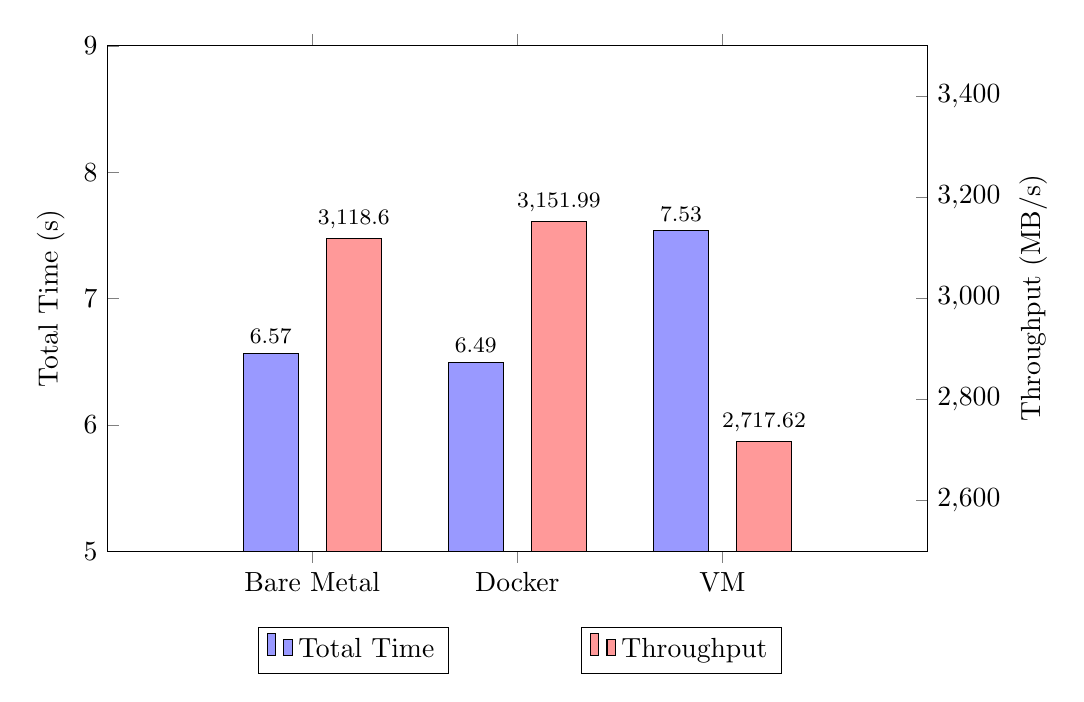
\begin{tikzpicture}
        \begin{axis}[
            ybar,
            bar width=20pt,
            bar shift=-15pt,
            width=12cm,
            height=8cm,
            enlarge x limits=0.5,
            ymin=5, ymax=9,
            ylabel={Total Time (s)},
            symbolic x coords={Bare Metal, Docker, VM},
            xtick=data,
            nodes near coords,
            nodes near coords align={vertical},
            nodes near coords style={font=\footnotesize},
            axis y line*=left,
            legend style={at={(0.3,-0.15)}, anchor=north}
        ]
        \addplot[fill=blue!40] coordinates {(Bare Metal, 6.5659) (Docker, 6.4933) (VM, 7.5349)};
        \addlegendentry{Total Time}
        \end{axis}

        \begin{axis}[
            ybar,
            bar width=20pt,
            bar shift=15pt,
            width=12cm,
            height=8cm,
            enlarge x limits=0.5,
            ymin=2500, ymax=3500,
            ylabel={Throughput (MB/s)},
            symbolic x coords={Bare Metal, Docker, VM},
            xtick=data,
            nodes near coords,
            nodes near coords align={vertical},
            nodes near coords style={font=\footnotesize},
            axis y line*=right,
            axis x line=none,
            legend style={at={(0.7,-0.15)}, anchor=north}
        ]
        \addplot[fill=red!40] coordinates {(Bare Metal, 3118.60) (Docker, 3151.99) (VM, 2717.62)};
        \addlegendentry{Throughput}
        \end{axis}
        
    \end{tikzpicture}
    \caption{مقایسه با بنچمارک \lr{Memory Intensive}}
\end{figure}       

\subsubsection{تحلیل نتایج}
طبق پیش‌بینی عملکرد \lr{Bare Metal} و Docker به شدت به هم نزدیک هست، در حالی که زمانی کل ماشین مجازی
بیشتر بوده و Throughput کمتری ثبت کرده است؛ در واقع کارایی کمتری داشته است.


\subsection{\lr{IO Intensive}}
\subsubsection{توضیح محک}
در این محک، ۴ گیگابایت فایل در دیسک ساخته می‌شود و سپس به صورت متوالی دستورات نوشتن بر این فایل‌ها
اجرا می‌شود، با توجه به کم بودن کارکرد CPU و تمرکز اصلی بر دیسک به جای حافظهٔ اصلی، این محک عملکرد
I/O را بررسی می‌کند.


\subsubsection{پیش‌بینی}
توقع می‌رود که \lr {Bare Metal} به این دلیل که هیچ لایهٔ میانی و سربار اضافی ندارد و مستقیما به فایل‌سیستم درخواست می‌زند،
بهترین عملکرد را داشته باشد (البته این سربار جزئی است و توقع می‌رود تقریبا 
کارایی مشابهی داشته باشند)، پس از آن Docker به دلیل حضور لایهٔ میانی با سربار جزئی، در رتبهٔ دوم باشد،
و سپس ماشین مجازی بدترین عملکرد را خواهد داشت، ماشین مجازی حق استفاده مستقیم از I/O را ندارد و باید درخواست از طریق شبیه‌سازی
لایهٔ رابط\footnote{Hyperviser} اتفاق بیفتد و به این دلیل به مراتب کندتر است.



\subsubsection{شبیه‌سازی}\begin{figure}[ht]
    \centering
    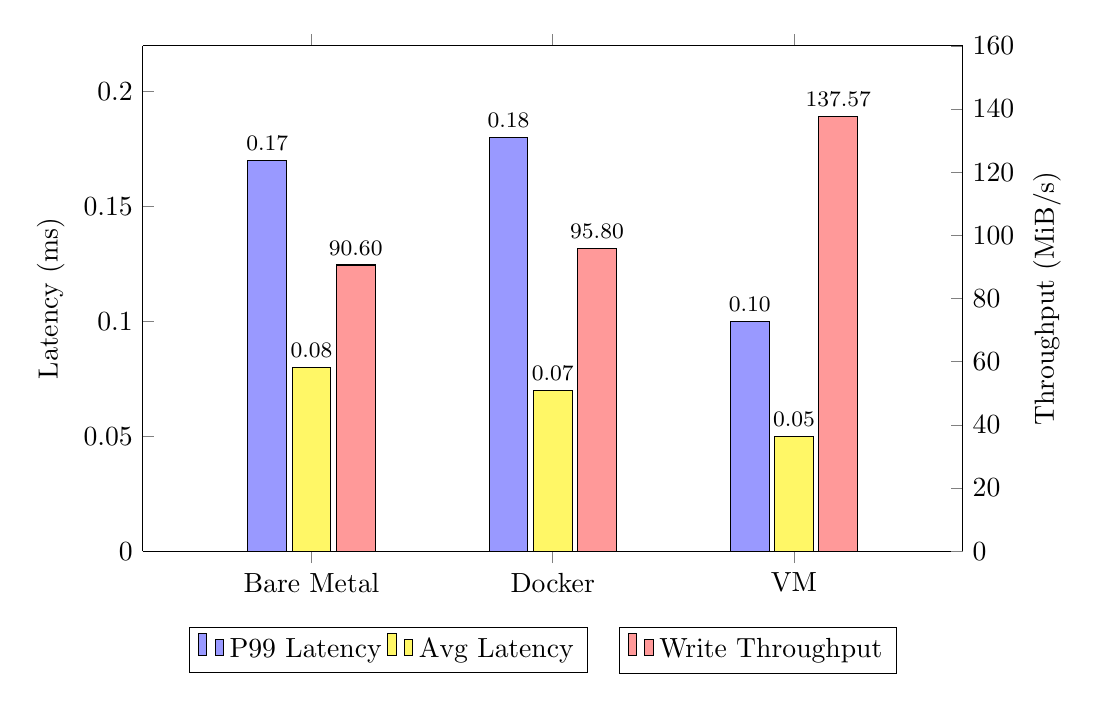
\begin{tikzpicture}
        \begin{axis}[
            ybar,
            bar width=14pt,
            width=12cm,
            height=8cm,
            enlarge x limits=0.35,
            ymin=0, ymax=0.22,
            ylabel={\lr{Latency (ms)}},
            symbolic x coords={Bare Metal, Docker, VM},
            xtick=data,
            yticklabel style={
                /pgf/number format/fixed,
                /pgf/number format/precision=2
            },
            nodes near coords,
            nodes near coords align={vertical},
            nodes near coords style={
                font=\footnotesize,
                /pgf/number format/fixed,
                /pgf/number format/fixed zerofill,
                /pgf/number format/precision=2
            },
            axis y line*=left,
            legend style={at={(0.3,-0.15)}, anchor=north, legend columns=2}
        ]
        \addplot[fill=blue!40, bar shift=-16pt] coordinates {(Bare Metal, 0.17) (Docker, 0.18) (VM, 0.10)};
        \addplot[fill=yellow!60, bar shift=0pt] coordinates {(Bare Metal, 0.08) (Docker, 0.07) (VM, 0.05)};
        \legend{\lr{P99 Latency}, \lr{Avg Latency}}
        \end{axis}

        \begin{axis}[
            ybar,
            bar width=14pt,
            width=12cm,
            height=8cm,
            enlarge x limits=0.35,
            ymin=0, ymax=160,
            ylabel={\lr{Throughput (MiB/s)}},
            symbolic x coords={Bare Metal, Docker, VM},
            xtick=data,
            nodes near coords,
            nodes near coords align={vertical},
            nodes near coords style={
                font=\footnotesize,
                /pgf/number format/fixed,
                /pgf/number format/fixed zerofill,
                /pgf/number format/precision=2
            },
            axis y line*=right,
            axis x line=none,
            legend style={at={(0.75,-0.15)}, anchor=north}
        ]
        \addplot[fill=red!40, bar shift=16pt] coordinates {(Bare Metal, 90.60) (Docker, 95.80) (VM, 137.57)};
        \addlegendentry{\lr{Write Throughput}}
        \end{axis}
    \end{tikzpicture}
    \caption{مقایسه با بنچمارک \lr{IO Intensive}}
\end{figure}

\subsubsection{تحلیل نتایج}
مطابق انتظار داکر و \lr{Bare Metal} عملکرد مشابهی دارند، لیکن ماشین مجازی علیرغم انتظار
عملکرد خیلی بهتری ارائه داده است؛ این احتمالا به این دلیل خواهد بود که درخواست نوشتن در دیسک توسط
سیستم عامل میهمان به درستی ارزیابی نمی‌گردد. به طور کلی موقع درخواست نوشتن در دیسک، در سطح سخت‌افزار
داده‌ها ابتدا در \footnote{Page Cache} نوشته شده و سپس به دیسک انتقال داده می‌شوند، هنگامی که بنچمارک در سیستم عامل
میزبان اجرا می‌شود درخواست می‌دهد که زمان سیگنال وضعیت پس از نوشتن کامل در دیسک برگردانده شود، در حالی که در سیستم عامل میهمان،
پردازه توانایی این را ندارد که حافظهٔ نهان سیستم عامل میزبان را دور بزند و به همین دلیل عملکرد بهتری نسبت به سیستم عامل
میهمان نشان خواهد داد؛ به عبارت دیگر در ماشین مجازی همچنان درحالی که داده در دیسک ذخیره نشده است، سیگنال اتمام کار دریافت می‌شود.